\clearpage
\section{Absorptionskoeffizient}
\label{section:Absorbtionskoeff}

\subsection{Linearer Absorptionskoeffizient}

Zur Bestimmung des Massenabsorptionskoeffizienten vom Aluminium, Eisen und Blei stellen wir jeweils 
unterschiedlich dicke/viele Stücke Abschirmmaterial zwischen Probe und Detektor. Als Präperat verwendet man Cs-137. Dann misst man jeweils das Spektrum und 
integriert die Counts dann über die Spektrallinie hinweg auf. Dabei werden immer mindestens 1000 Counts unter dem Integral abgewartet, 
um ein Signal-Rausch-Verhältnis von über 10 aufgrund der Poisson-Statistik zu erhalten. \\
Zuerst messen wir dabei immer ohne Abschirmmaterial, aber mit Abstandshalter – ein Rohr mit circa 15\,cm Länge. In diesen legen wir dann das Abschirmmaterial und messen dieses aus. 
Dabei nehmen wir mehr Messwerte bei dünner Abschirmdicke $d$, da diese messzeitminimierned ist und dadurch die Anzahl an insgesamt detektierten Zerfällen höher ist, was das Signal-Rausch-Verhältnis verbessert. \\
Gemessen wurde in der Reihenfolge Aluminium, Eisen, Blei und als Integralgrenzen wurden die Töpfe 442 und 451 verwendet.

Die Intensität der Gammastrahlung verhält sich dabei in Abhängigkeit der Dicke wie folgt:

\begin{equation}
    I = I_0 \exp(- \mu d) +I_R
    \label{Intensitaet}
\end{equation}

$I_0$ = Intensität vor Absorber, $I_R$ = Intensität des Rauschens, $\mu$ = linearer Absorptionskoeffizient, $d$ = Absorberdicke. 

Aus dem obigen Integral und der gemessenen Zeit kann man dann eine Zählrate ermitteln. Diese ist direkt proportional zur Intensität. 
Aus dieser und den Absorberdicken kann man dann numerisch mit der Methode der kleinsten Quadrate die optimalen Parameter bestimmen. Außerdem kann man 
noch den Fehler durch das Schätzen des Parameters abschätzen. Dies macht der Computer indem er die Funktion nimmt 
und den Parameter variiert. Damit ein Parameter mit der Messung vereinbar ist, 
muss die Wahrscheinlichkeit das Messergebnis zu erhalten über einem bestimmten Signifikanzniveau liegen.\\

\subsubsection*{Aluminium}

Für Alu ergibt sich folgender Verlauf wie in Abbildung \ref{AbsorbtionkoeffAlu} zu sehen.\\

\begin{figure}[ht]
    \centering
    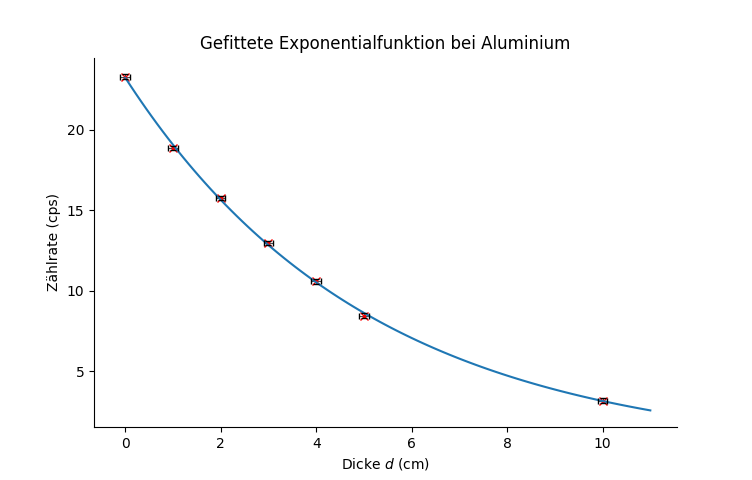
\includegraphics[width = \linewidth]{Bilder/Auswertung/AbsorbtioskAlu.png}
    \caption{Zählrate bei jeweiliger Absorberdicke $d$}
    \label{AbsorbtionkoeffAlu}
\end{figure}

 
Der durch den Fit angegebene Fehler beinhaltet schon die Messfehler, da diese in der Abweichung der Daten vom theoretischen Modell 
schon enthalten sind.
\begin{center}
    \centering
    \textcolor{red}{$\mu_{Alu}= (0,20 \pm 0,02) \mathrm{cm}^{-1}$}
\end{center}

Da die Fehlerbalken der Punkte in Abbildung \ref{AbsorbtionkoeffAlu} so klein sind, werden diese bei den folgenden Grafiken weggelassen. 
\subsubsection*{Eisen}
Bei Eisen wird wie oben vorgegangen. Dabei ergibt sich folgender Kurvenverlauf (Abbildung \ref{AbsorbtionkoeffFe}). Dabei ist schon am Graphen eindeutig eine stärkere Abschirmung zu sehen. Diese spiegelt sich dementsprechend 
auch in dem linearen Absorptionskoeffizient wieder.


\begin{center}
    \centering
    \textcolor{red}{$\mu_{Fe}= (0,53 \pm 0,05) \mathrm{cm}^{-1}$}
\end{center}

\subsubsection*{Blei}

Bei diesem Teil könnte der Fehler zu klein abgeschätzt sein, da die verwendeten Bleiplatten in ihrer Dicke stark variiert haben. Daher kann es zu einem 
systematischen Fehler kommen, da die Anzahl der Absorberplättchen erfasst wurde, nicht aber die Gesamtdicke. Diese wurde einmal gemessen und mit der 
errechneten Dicke abgeglichen. Dabei wich diese um 50\% ab. Die kann unteranderem an Luft zwischen den nicht ebenen Plättchen liegen, aber auch an Dickeunterschieden.\\
Wie oben ist nochmal eine deutliche Zunahme des Absorptionsvermögens zu sehen. Dies liegt unter anderem an der höheren Dichte von Blei und dem höheren 
Wirkungsquerschnitt durch die höhere Kernladungszahl, welche sich in einem schnelleren Abfall der Kurve in Abbildung \ref{AbsorbtionkoeffPb} wiederspiegelt.

\begin{center}
    \centering
    \textcolor{red}{$\mu_{Pb}= (1.1\pm 0.1) \mathrm{cm}^{-1}$}
\end{center}

\subsection{Massenabsorptionskoeffizient}

Der Massenabsorptionskoeffizient $\frac{\mu}{\rho}$ ist eine Größe, welche den linearen Absorptionskoeffizienten $\mu$ in Verbindung mit der Dichte $\rho$ des Materials setzt.
Man kann ihn also auch als Maß für den Wirkungsquerschnitt der Atome verstehen. Je größer der Massenabsorptionskoeffizient, desto wahrscheinlicher ist es für einen 
Nukleon von der Strahlung 'getroffen' zu werden. 

\begin{center}
    \centering
    \textcolor{red}{$\frac{\mu_{Al}}{\rho_{Al}} = (0,073 \pm 0,005) \mathrm{cm}^{2} \mathrm{g}^{-1}$}\\
    \textcolor{red}{$\frac{\mu_{Fe}}{\rho_{Fe}}= (0,068 \pm 0,006) \mathrm{cm}^{2} \mathrm{g}^{-1}$}\\
    \textcolor{red}{$\frac{\mu_{Pb}}{\rho_{Pb}}= (0,101 \pm 0,009) \mathrm{cm}^{2} \mathrm{g}^{-1}$}\\
\end{center}

Hierbei wurde für $\rho_{Al} = 	2,6989 \frac{\mathrm{g}}{\mathrm{cm}^3}$, $\rho_{Fe} = 	7,874 
\frac{\mathrm{g}}{\mathrm{cm}^3}$ und
$\rho_{Pb} = 11,342 \frac{\mathrm{g}}{\mathrm{cm}^3}$  verwendet (\cite{CRC1990}).\\
Man sieht schön, dass der Wirkungsquerschnitt mit steigender Kernladungszahl stark ansteigt.


